\begin{abstract}
  We present a platform for Melanoma Classification, leveraging a technical
  infrastructure based on Convolution Neural Network (CNN) models based on
  ResNet18.

  For training and validation, exclusively we have utilized image data, and no
  additional metadata is incorporated during the training process. Various
  training strategies, such as data augmentation, learning rate decay, dropout,
  etc., were employed to enhance models performance.

  The resulting models are accessible through a  API, enabling users to
  interact with them via a straightforward web application. Users can submit
  batches of images to the API for classification, contributing to a
  user-friendly experience.

  This platform demonstrates the efficacy of CNNs in melanoma classification,
  highlighting the importance of diverse training approaches. The API provides
  a practical interface for users to seamlessly integrate melanoma
  classification into their workflows.
\end{abstract}


\section{Introduction}

Skin cancer, including melanoma, is a significant global public health concern.
Melanoma presents a considerable challenge due to its high mortality rate and
the critical importance of early detection for successful treatment. Cancer
begins when healthy cells undergo changes that cause them to grow and divide
uncontrollably, forming tumors. These tumors can be classified as either
cancerous (malignant) or non-cancerous (benign). \\

In recent times, there has been a growing focus on automating tasks in the
medical field through Computer-Aided Diagnosis (CAD)\footnote{CAD refers to the
use of computer algorithms and technologies to assist healthcare professionals
in the process of medical diagnosis.}. Some studies have demonstrated that
these systems can achieve results similar to those of professionals. However,
the integration of CAD into the medical system remains a significant challenge. \\

The development of a CAD system necessitates the creation of models capable of
effectively classifying melanoma. The SIIM-ISIC Melanoma Classification
challenge specifically tasks participants with building models for identifying
melanoma using skin lesion images and associated metadata. This thesis outlines
our approach, wherein we leverage data from this challenge to train our models
and subsequently expose them through our platform. By doing so, we contribute
to the ongoing efforts to bridge the gap between cutting-edge medical imaging
technology and practical clinical applications.

\newpage

\section{Objectives}

The final objective of this thesis is to craft a CAD infrastructure,
focused on melanoma detection using deep learning vision models capable of detecting melanoma on dermoscopy images. To this end, the gradual achievements that
must be accomplished are:

\begin{itemize}

  \item Gaining a comprehensive understanding of the theory
    behind deep learning vision models and its practical applications.

   \item Select a base transfer model. Is the model good enough?, the selection of this model is given by the technical limitations?, or any other justification.

  \item Study different approaches to train the models and select a good  evaluate metric given the dataset distribution of dermoscopy images.

  \item  Develop the CAD infrastructure. It should contain
    the  trained models, a simple web UI\footnote{User Interface. Is
    the point of human-computer interaction and communication in a device.}, an
    API\footnote{Application Programming Interface. Is a set of protocols,
      routines, tools, and definitions that allow different software applications
    to communicate with each othe} and finally a mechanism using Docker to create
    the images of these services making it ease to deploy in any based Linux System.

\end{itemize}


\section{Development process}

The project methodology employed in this endeavor follows a continuous process.
The project incorporates the concept of utilizing idle time effectively. For
instance, during the training of models, there are periods of idle time, which
we exploited by concurrently working on other tasks related to developing the
entire infrastructure. This approach allows for maximizing productivity
throughout the project, see Figure \ref{fig:flux_development}.

\newpage

\begin{landscape}

  \begin{figure}[H]
  \centering
  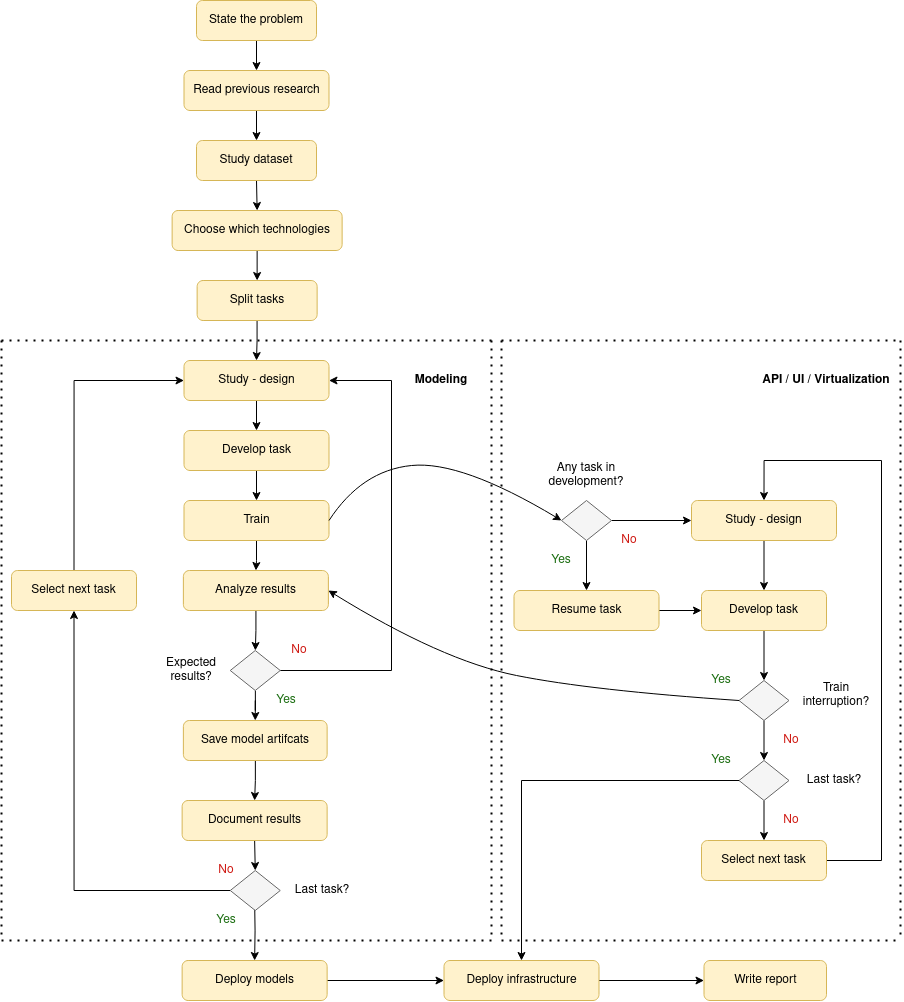
\includegraphics[width=0.82\textwidth]{imatges/planing_and_methodology/EmplyedMethodology.png}
  \caption{\textit{Development process methodology.}}
  \label{fig:flux_development}
  \end{figure}

\end{landscape}

\newpage

\section{CAD infrastructure pipeline}

Our CAD infrastructure pipeline  (see Figure \ref{fig:cad-pipeline}), consists
of different steps, beginning with data acquisition, followed by data
preprocessing. We then set up different datasets for training, validation, and
testing. Subsequently, we train the models and, assess the models gathering
metrics and finally we deploy the models under an API.

\begin{figure}[H]
  %\begin{adjustbox}{width=\textwidth, trim={0.2cm 0pt 1.5cm 0pt}, clip}
  \centering
  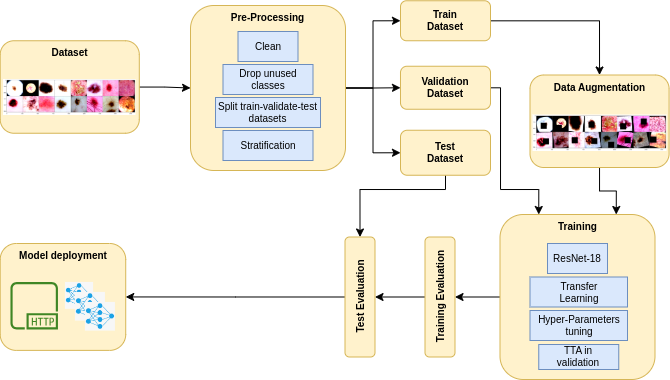
\includegraphics[width=0.9\textwidth]{imatges/methodological_contribution/Pipeline.drawio.png}
  %\end{adjustbox}
  \caption{\textit{CAD infrastructure pipeline. Train, test and deploy. }}
  {\label{fig:cad-pipeline}}
\end{figure}

\section{Data and training strategies}

Inspired by the approach of the Winning Solution to the SIIM-ISIC Melanoma
Classification Challenge \cite{WinningISIC}. The Winning Solution team observed
that in the entire dataset of 2020, comprising 33K images, only 1.76\% were
positive samples (i.e., malignant). In response, they decided to augment this
data by incorporating information from the datasets of the same competition
from the previous years (2018 and 2019). Although the individual datasets from
these earlier years were smaller, totaling 25K images, they exhibited a
positive ratio of 17.85\%. This strategic combination allowed for a more
balanced representation of positive cases in the training data. \\

To build the original dataset, we utilized 8 classes selected from the raw
dataset, as the remaining classes we considered not significant or there were
very few samples of them. Any sample that was not categorized as one of the
following classes were excluded from the training process.

\begin{itemize}
  \item melanoma
  \item nevus
  \item BCC (Basal Cell Carcinoma)
  \item BKL (Benign lesions of the keratosis)
  \item AK (Actinic Keratosis)
  \item SCC (Squamous Cell Carcinoma)
  \item VASC (Vascular Lesions)
  \item DF (Dermatofibroma)
\end{itemize}

The filtered dataset comprises 31,265 distinct image samples, demonstrating a
highly imbalanced dataset, as evident from Figure
\ref{fig:hole-dataset-distribution}.

\begin{figure}[H]
  \centering
  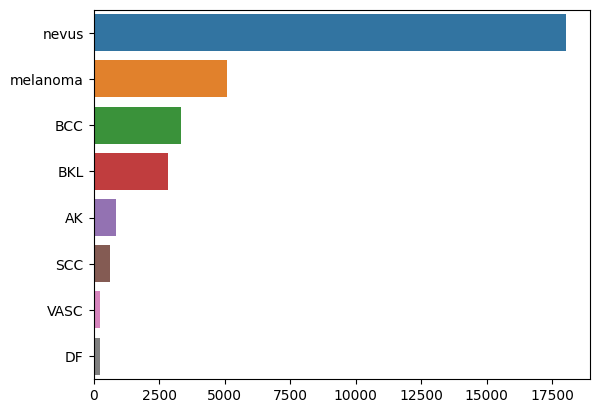
\includegraphics[width=0.75\textwidth]{imatges/data-training-strategies/hole-dataset-diagnosis.png}
  \caption[Categories distribution in dataset]{\textit{Categories distribution in dataset.}}
  {\label{fig:hole-dataset-distribution}}
\end{figure}


We started dividing the original dataset into three subsets using the Holdout
set scheme, see Figure \ref{fig:holdout-test-scheme}. \\

During the training phase, the test set remains completely separate and is not
used in any way to configure the hyper-parameters. This ensures that the
performance of a model on the test set is not artificially inflated by
adjusting hyper-parameters to achieve an exceptionally good outcome in the validation set. \\

\newpage

The data from the ISIC Archive was divided using the following percentages: 80\%
for training, 10\% for validation, and 10\% for testing. Each subset contain the same
distribution of classes as the original dataset, i.e., we applied stratification.

\begin{figure}[H]
  \centering
  \begin{adjustbox}{width=0.7\textwidth, trim={0cm 1cm 0cm 1.25cm}, clip}
    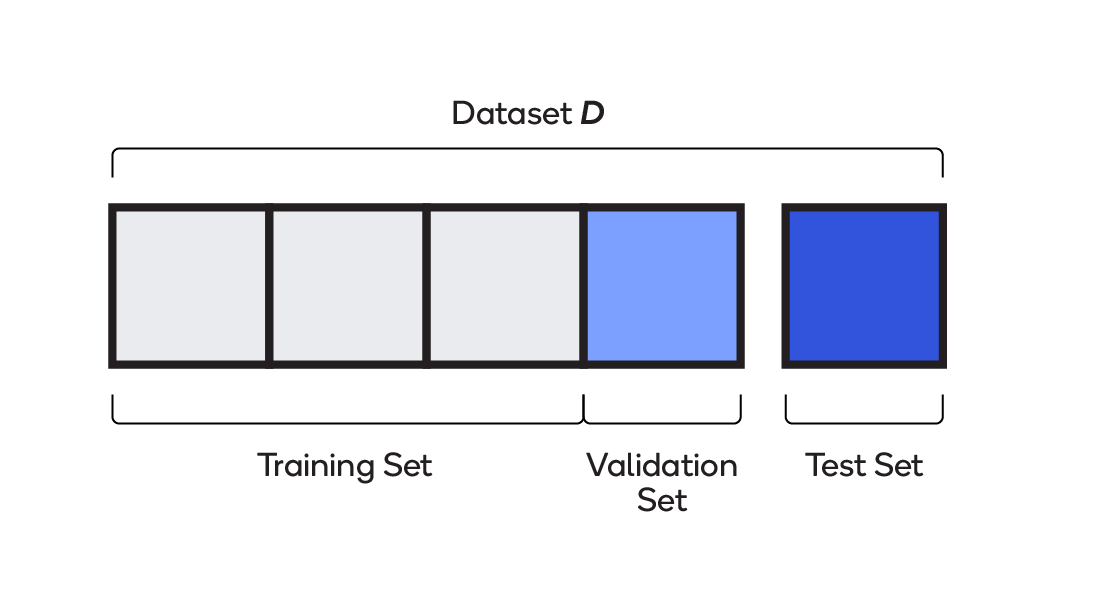
\includegraphics[width=\textwidth]{imatges/data-training-strategies/train-test-validation-sets.png}
  \end{adjustbox}
  \caption[Holdout set scheme]{\textit{Holdout set scheme. Illustration by Qualcomm}}
  {\label{fig:holdout-test-scheme}}
\end{figure}

In small to medium sized datasets, augmentation is important to prevent
overfit. For some of our trained models, we used in the training dataset our
augmentation pipelines, as illustrated in Figure \ref{fig:sample-of-datasets} and
Figure \ref{fig:aug-sample-of-datasets}, with contains the following augmentations
from the popular and powerful PyTorch augmentation library Albumentations
\cite{Albumentations}: Transpose, Flip, Rotate, RandomBrightness,
RandomContrast, MotionBlur, MedianBlur, Gaus- sianBlur, GaussNoise,
OpticalDistortion, GridDistortion, ElasticTransform, CLAHE, HueSaturationValue,
ShiftScaleRotate, Cutout.

\begin{figure}[H] \centering
  \begin{adjustbox}{width=0.9\textwidth}
    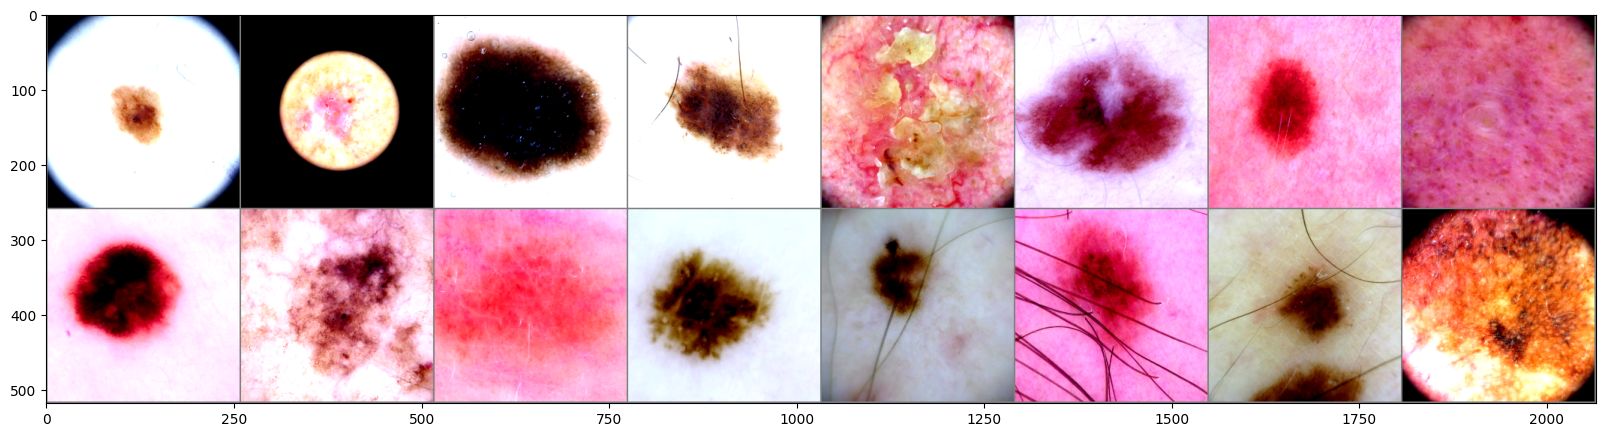
\includegraphics[width=\textwidth]{imatges/methodological_contribution/random-sample-of-isic.png}
  \end{adjustbox}
  \caption[Random sample of images]{\textit{Random sample of images.}}
  {\label{fig:sample-of-datasets}}
\end{figure}

\begin{figure}[H]
  \centering
  \begin{adjustbox}{width=0.9\textwidth}
  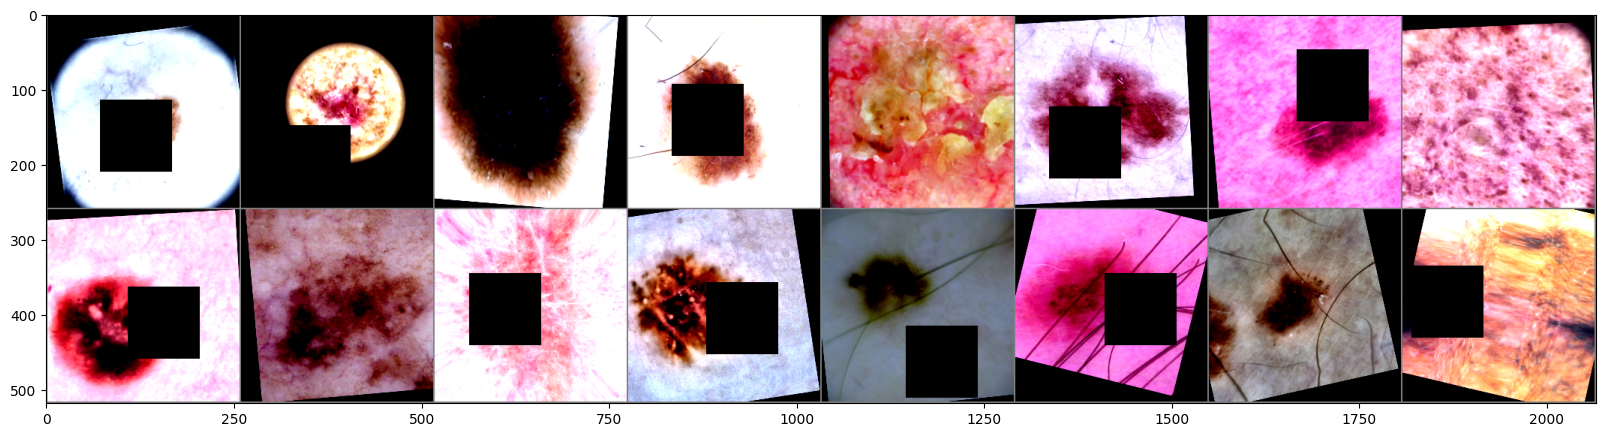
\includegraphics[width=\textwidth]{imatges/methodological_contribution/random-sample-of-isic-augmented.png}
  \end{adjustbox}
  \caption[Augmented random sample of images]{\textit{Augmented random sample of images.}}
  {\label{fig:aug-sample-of-datasets}}
\end{figure}


We decided to use as transfer model an already trained ResNet in the ImageNet
database. ResNet is short for "Residual Network," is a deep convolutional
neural network (CNN) architecture that was introduced in 2015 by researchers
from Microsoft Research \cite{ResNetPaper}. It revolutionized the field of deep
learning by addressing the challenge of training very deep neural networks. \\

There are various architectural variants or "flavors" of ResNet, including
ResNet-152,  ResNet-101,  ResNet-50,  ResNet-34, and  ResNet-18. The number
following the name of each ResNet variant indicates the number of inner layers
present in the architecture. The more the number of the layers the more the
accuracy, yet the number of parameters to be trained increase. To accurately
assess the performance of each ResNet architecture, refer to Table
\ref{table:resnet}, which provides the accuracy achieved on the ImageNet
dataset along with the corresponding number of trainable parameters in
millions.

\begin{table}[H]
  \centering
  \begin{tabular}{lcc}
    \toprule
    \textbf{Model} & \textbf{Accuracy} & \textbf{Parameters} \\
    \midrule
    ResNet-152 & 78.31\% & 60.2M \\
    ResNet-101 & 77.37\% & 44.5M \\
    ResNet-50 & 76.15\% & 25.6M \\
    ResNet-34 & 73.30\% & 21.8M \\
    ResNet-18 & 69.76\% & 11.7M \\
    \bottomrule
  \end{tabular}
  \caption[Accuracy achieved on ImageNet and trainable parameters of each ResNet]
  {\textit{Accuracy achieved on ImageNet and trainable parameters of each ResNet.
  Each image in the ImageNet dataset is associated with 1 of 1,000 classes. Table by paperswithcode}}
  {\label{table:resnet}}
\end{table}

We decided to use ResNet18 as base model only for technical reasons. The lack
of powerfull GPUs took us to pick this estimator agains the others. There are
other architectures that we could have tried as: AlexNet, ResNetXt, VGG, etc,
but comparing the performance of those models in the SIIM-ISIC Melanoma
competition is not the goal of this thesis.

\section{Validation strategy}

In any machine learning project, it is critical to establish a reliable
validation scheme to properly evaluate and compare models. This becomes
particularly crucial when dealing with a small to medium-sized dataset or when
the evaluation metric is unstable, as is the case with the dataset provided in
the competition. There are various metrics commonly used to assess the quality of a model's
predictions. We present a selection of metrics that we find relevant for
evaluating our models. \\

A confusion matrix (see Figure \ref{fig:confusion-matrix}) is a square matrix
with dimensions {\tt NxN}, where {\tt N} represents the total number of classes being
predicted.

\begin{figure}[H]
  \begin{adjustbox}{trim={0pt 0.5cm 0pt 1cm}, clip}
    \centering
    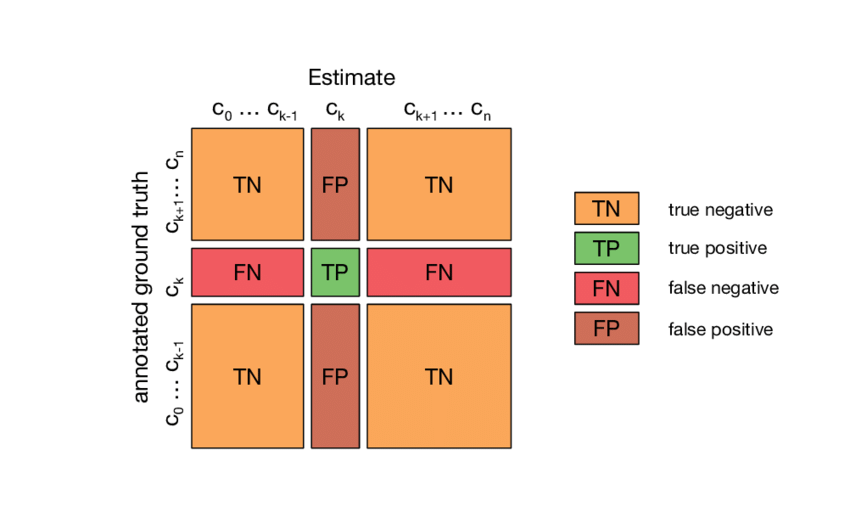
\includegraphics[width=0.9\textwidth]{imatges/validation-strategy/confusion-matrix.png}
  \end{adjustbox}
  \caption[Confusion matrix multi-class]{\textit{Confusion matrix multi-class. Illustration by kaggle}}
  {\label{fig:confusion-matrix}}
\end{figure}

From confusion matrix we can obtain other metrics such as:

\begin{itemize}

  \item {\bf Accuracy}

    The Accuracy metric, calculates the ratio of correct predictions to the total number of
    predictions made on a dataset. It is not a good matric when working with
    unbalanced datasets.

    \[Accuracy = \frac{TP + TN}{TP + TN + FP + FN}\]

  \item {\bf True Positive Rate (TPR) or Sensitivity}

    The True Positive Rate tells about how many of the true class samples were
    correctly classified.

    \[TPR = \frac{TP}{TP + FN}\]


  \item {\bf False Positive Rate (FPR) or False Alarm Ratio}

    The False Positive Rate tells the proportion of the true class samples that
    were not correctly classified and are False Positive.

    \[FPR = \frac{FP}{FP + TN}\]


  \item {\bf Receiver Operator Characteristic (ROC)}

	  An ROC curve plots TPR vs. FPR at different classification thresholds {\tt
	  T}, where $T \ \text{for} \ 0 <= x <= 1$. Lowering the classification
	  threshold classifies more items as positive, thus increasing both False
	  Positives and True Positives. By plotting the curve, you can say which
	  threshold is better, depeding on how many False Positive we are willing to
	  accept.

    \begin{figure}[H]
      \centering
      \begin{adjustbox}{trim={0pt 0cm 0pt 0cm}, clip}
        \centering
        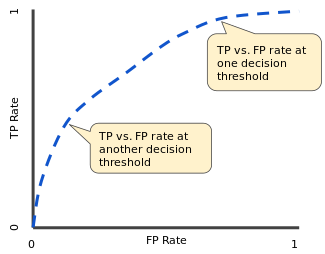
\includegraphics[width=0.55\textwidth]{imatges/validation-strategy/ROCCurve.png}
      \end{adjustbox}
        \caption{\textit{Typical ROC Curve. Illustration by Alphabet Inc.}}
      {\label{fig:ROCCurve}}
    \end{figure}


  \item {\bf Area Under the Curve (AUC)}

  The Area Under the Curve is a value between 0 and 1 that measures the
  ability of a classifier to distinguish between classes. It is used as a summary of
  the ROC curve. The higher the AUC, the better the performance of the model at
  distinguishing between the positive and negative classes.

  \begin{figure}[H]
    \centering
    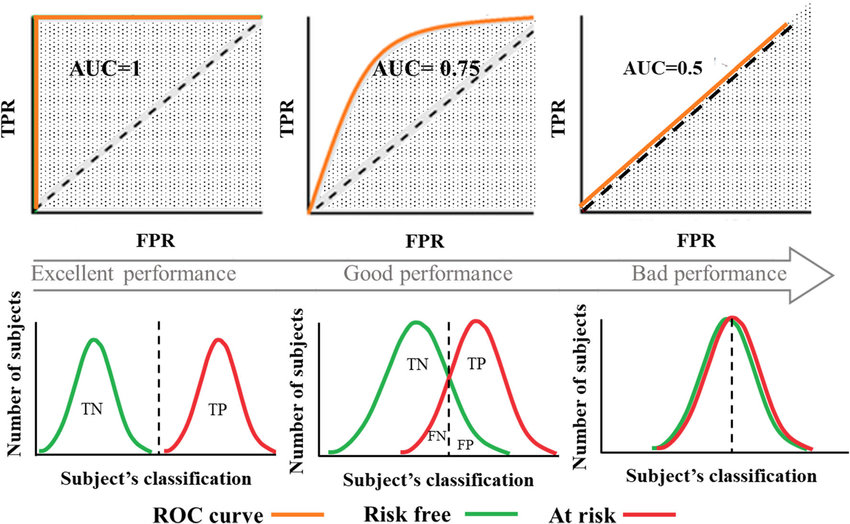
\includegraphics[width=0.7\textwidth]{imatges/validation-strategy/auc.png}
    \caption[AUC-ROC performance]{\textit{AUC comparation. Illustration by Elizabeth Louise Thomas}}
    {\label{fig:auc-roc}}
  \end{figure}

\end{itemize}

\newpage

\section{Models metrics}

The training phase ended with the development of eight models using an
imbalanced dataset comprising eight classes. Various learning policies and
Artificial Intelligence (AI) techniques were tested during the experimentation
process.

These models were divided into two categories: one without any
additional regularization and another with additional regularization techniques
such as data augmentation and the inclusion of dropout layers.

\begin{table}[H]
\centering
\begin{tabular}{lc|lc}
    \toprule
  \textbf{Model} & \textbf{Test AUC} & \cellcolor{gray!50}\textbf{Model} & \cellcolor{gray!50}\textbf{Test AUC}  \\
\midrule
 M0 & 0.892 & \cellcolor{gray!50}M4 & \cellcolor{gray!50}0.858 \\
 M1 $\star$ & 0.892 & \cellcolor{gray!50}M5 $\star$ & \cellcolor{gray!50}0.843 \\
 M2 $\ast$ &  0.885 &  \cellcolor{gray!50}M6 $\ast$ & \cellcolor{gray!50}0.848 \\
 M3 $\bullet$ & 0.886 & \cellcolor{gray!50}M7 $\bullet$ & \cellcolor{gray!50}0.849 \\
 \midrule
Mean &  88.875\% & \cellcolor{gray!50}Mean & \cellcolor{gray!50}84.950\%  \\
SD &  0.377\%  &   \cellcolor{gray!50}SD &  \cellcolor{gray!50}0.625\%  \\

\bottomrule
\end{tabular}
\caption[Models metrics in test dataset]
  {\textit{Models metrics in test dataset.}}
{\label{table:test-set-resume-metrics}}
\end{table}

The initial group of models performed well on the test set with an average AUC
of 88.875\% and a small standard deviation of ±0.377\%. However, they showed
signs of overfitting on the validation set. In contrast, the second group of
models, trained with additional regularization techniques, achieved lower
results but did not suffer from overfitting. They had an average AUC of 84.950%
with a standard deviation of ±0.625\%, which was influenced by more training
epochs.

During model training, we also developed the necessary CAD infrastructure. For
the API, we used a flexible approach with soft configurations that could be
specified through file-based parameters, offering adaptability and simplified
management. Additionally, we created an intuitive UI for seamless interaction
between healthcare professionals and the models.

We also provided a Docker-based script for easy deployment of the
infrastructure on any Linux operating system, ensuring efficient startup and
operation.

\section{CAD infrastructure result}
